%!TEX root = ./Structure_rapport_final.tex


\subsection{Sampling and specimens}

This study used fishes that were collected during Ifremer's EVHOE (EValuation Halieutique de l'Ouest Européen) research cruises, surveying the Bay of Biscay every fall onboard the \textit{R/V Thalassa}.
Several hauls are performed each night, so the whole campain surveys several stations. Each station is precisely defined with its GPS coordinates and located above canyons, at the the edge of continental shelf. If they are considered to be ``biodiversity hotspot'', canyons communities are yet relatively unknown, because of the logistic and material difficulties that their exploration implies \citep{gillet2013}.
To sample bathypelagic fishes, pelagic trawling is performed during night, between 700 and 2000 meters, because those fishes perform diel vertical migrations and tends to come closer to the surface at nighttime. To this end, 25 meters-wide opening trawl is used, with as mesh size decreasing from 76mm to 48mm at the end of the trawl, at a toing speed of 4 knots for about an hour. 
Once the trawl is pulled back onboard, fishes are sorted, identified, up to species when possible, and frozen, and then stock into sample banks when the campain is over. 

For this study, only abundant-enough species that can thus be considered as common in Biscay Bay deep seas, are treated, leading to a total of 9. All teleost, 4 of them belong to the Microphidae (lanternfish) family, which is the most abundant and widely spread family across all oceans \citep{debusserolles2014} and could represent up to 65\% of the pelagic deep-sea biomass \citep{poulsen2013}: \textit{Lampanyctus crocodilus}, \textit{Myctophum punctatum}, \textit{Notoscopelus kroeyeri} \& \textit{Ceratoscopelus maderensis}. The second most represented family is the Platytrocidae, with 2 species: \textit{Searsia koefoedi} \& \textit{Normichthys operosus}. This family seems to be found in all oceans but not in Mediterranean Sea \citep{orrell2016}. Finally, 3 families are represented by one species each: \textit{Xenodermichthys copei} (Alepocephalidae); \textit{Arctozenus risso} (Paralepididae) \& \textit{Argyropelecus olfersii} (Sternoptychida), which are common species, found in every ocean \citep{carvalho1988,froese2019}.

\begin{figure} [!htbp]
	\begin{center}
		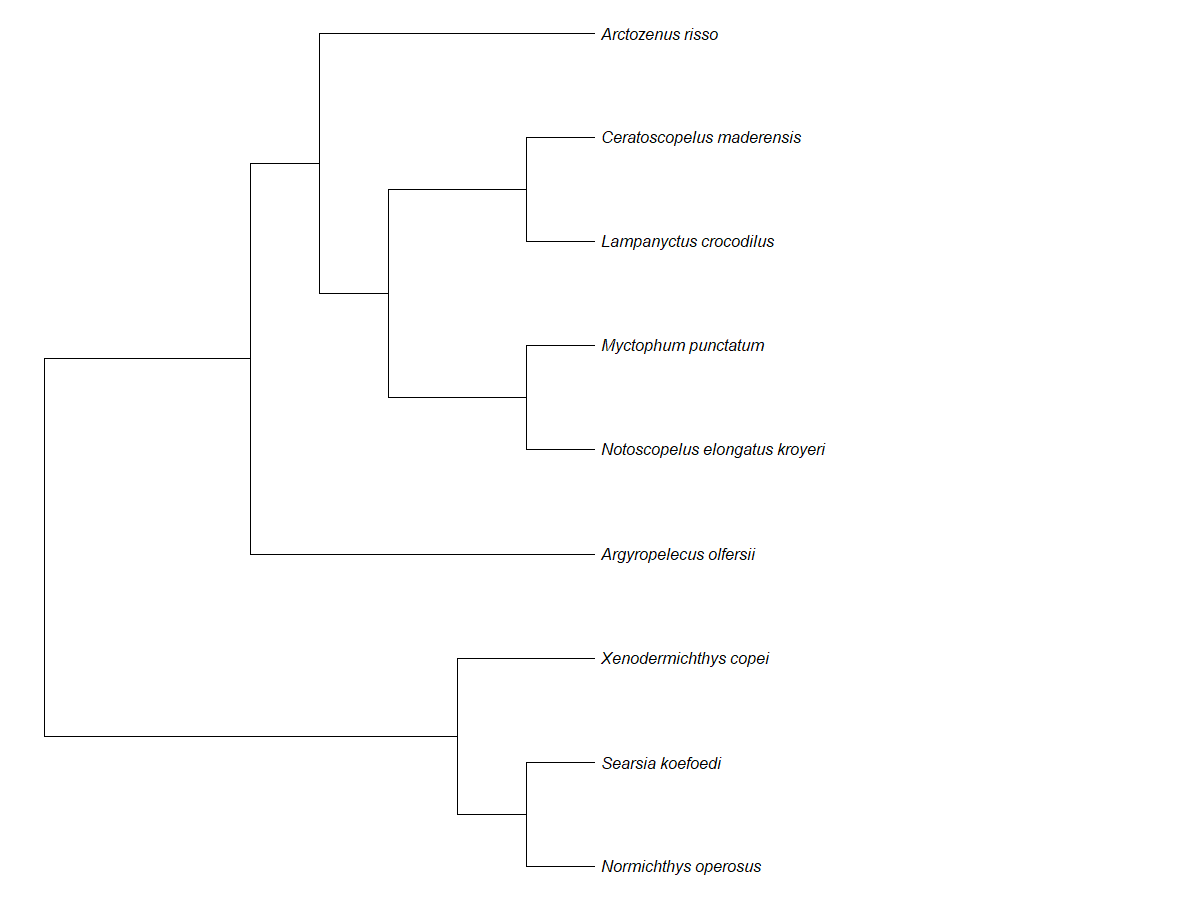
\includegraphics[width=0.8\textwidth]{phylogenic_tree.png}
	\end{center}
	\caption[Petite légende]{Phylogenic tree of studied species, using R \emph{rotl} package~\citep{opentreeoflife2019}~.}
	\label{fig:phylotree}
\end{figure}

\subsection{Morphological measurements and functional traits}
In lab, fish were thaw and 24 morphological measurements were taken on individuals, using an electronic caliper with a precision up to 0.01mm. Part of these measurements had previously been taken by students from La Rochelle Université during pratictal class. For the sake of statistical robustness and representativiy, at least 20 individuals were measured for each species. To this end, additional measurements were performed during this study leading to the individual number in Table \ref{table:spcount}.  

%Voir script table_tex.Rnw
\begin{table}[ht]
\centering
\caption{Species individual count and abundance}
\label{table:spcount}
\begin{tabular}{>{\itshape}lcc}
  \hline
Species & Count & Abundance (\%) \\ 
  \hline
Arctozenus risso &  20 & 7.75 \\ 
  Argyropelecus olfersii &  37 & 14.34 \\ 
  Lampanyctus crocodilus &  39 & 15.12 \\ 
  Myctophum punctatum &  25 & 9.69 \\ 
  Notoscopelus kroyeri &  36 & 13.95 \\ 
  Searsia koefoedi &   5 & 1.94 \\ 
  Xenodermichthys copei &  38 & 14.73 \\ 
  Ceratoscopelus maderensis &  20 & 7.75 \\ 
  Normichthys operosus &  38 & 14.73 \\ 
   \hline
\end{tabular}
\end{table}

Following what had been made on similar studies and according to our measurements, a total of 21 functional traits were computed from morphological measurements and informs on 3 main functions: food acquisition, swimming behavior and habitat (see Table \ref{table:functraits}).

\begin{sidewaystable}
\centering
\caption{Description and formulas of the functionals traits computed from morphological measurements, following \citep{albouy2011, aneeshkumar2017,boyle2006,brindamour2016,diderich2006,dumay2004,habib2019,ibanez2007,sibbing2000,webb1984,winemiller1991}. Abbreviations used in formulas are provided by raw measurements and detailed in appendices \ref{fig:app1}, \ref{fig:app2} \& \ref{fig:app3}. \textsc{oga}, \textsc{git}, \textsc{pc}, \textsc{pht} are categorial variables directly provided by raw measurements with \textsc{git} and \textsc{oga} scores detailed respectively in appendices \ref{fig:app4} \& \ref{fig:app5}.}
\label{table:functraits}
\begin{tabular}{>{\bfseries}lll>{\scshape}l}
  \hline
Function & Functional trait & Description & Formula  \\ 
  \hline
\multirow{13}{*}{Feeding} &Oral gape axis & Feeding position and depth in the water column & oga \\ 
  &Eye size & Detection of preys and visual acuity for predators & ed/hd \\ 
  &Orbital length & Preys size and behavior (buried, camouflaged) & ed/sl \\ 
  &Oral gape surface & Type and size of preys & mw*md / bw*bd \\ 
  &Oral gape shape & Strategy to capture prey & md/mw \\ 
  &Oral gape position & Fedding position in the water column & mo/hd \\ 
  &Lower jaw length & Compromise between power and opening speed of the mouth & ljl/sl \\ 
  &Gill raker type & Filtration capacities of fish & git \\ 
  &Gill outflow & Succion capacities of fish & ow \\ 
  &Operculum volume & Operculum volume (chercher à quoi ça sert) & od/ow \\ 
  &Head length & Maximum prey size & hl/sl \\ 
  &Pyloric caeca & Presence/Absence of pyloric caeca & pc \\ 
  &Anus position & Digestive tract length & pal/sl \\ 
  \hline
  \multirow{6}{*}{Locomotion} & Body depth & Swimming capacities of fish linked to their food prospection behavior & bd/sl \\ 
  &Pectoral fin position & Maneuvrability of fish & pfi/pfb \\ 
  &Pectoral fin insertion & Insertion de la pectorale (chercher à quoi ça sert) & ppl/sl \\ 
  &Transversal shape & Position in the water column and hydrodynamism & bd/bw \\ 
  &Caudal throttle width & Swimming strategy (cruiser/sprinter) & cpd \\ 
  &Dorsal fin insertion & Swimming behavior (chercher à quoi ça sert) & pdl/sl \\ 
  \hline
  \multirow{2}{*}{Others} &Eye position & Position in the water column (pelagic/sedentary) & eh/hd \\ 
  &Presence photophores & Presence/Absence of photophores (chercher à quoi ça sert) & pht \\ 
   \hline
\end{tabular}
\end{sidewaystable}

\subsection{Data analysis}
All data analysis were performed using \textsf{R} version 4.0.3 \citet{rcoreteam2021}.

\subsubsection{Data pre-processing}
Because measurements came from several observators, raw data had to be checked for outliers. To do so, data were standardised by \textsc{sl} and the interquartile range (IQR) method of outlier detection was applied to remove outliers ADD REF. According to this method, for each variable (measurement) and for each species, outliers are defined as every value outside this interval: 
\begin{center}
$ [Q1 - 1.5*QR, Q3 + 1.5*IQR]$ \\
with $Q1$ and $Q3$ being respectively first and third quartile, $IQR = Q3 - Q1$. 
\end{center}{}


Missing values that were previously present in the data set (\textit{n=28}) and those induced by outlier removal function (\textit{n=179}), are then imputed following k-Nearest Neighbor (kNN) method, which as proven to be effective ADD REF. Based on non-missing values points, kNN algorithm computes Euclidian distances between points, and assumes that missing value can be approximated by the values of points that are the closest. To this end \emph{tidymodels} R package and \emph{step\_knnimpute} function \citep{kuhn2020} were used, with a number of nearest neighbors (\textit{k}) of $\sqrt{N}$, with $N$ being the number of observations, i.e individuals, of the dataset. ADD ACCURACY OF PREDICTIONS? Accuracy was checked with linear regression of each variable with \textsc{sl}. Functional traits were computed on this full data set, using formulas in table \ref{table:functraits}. 

\subsubsection{Factorial Analysis of Mixed Data (FAMD)}
Because the data set contained a mix of qualitative and quantitative variables, FAMD method was used, which performs PCA (Principal Component Analysis) on quantitative variables and MCA (Multiple Correspondence Analysis) on qualitative variables. TROUVER COMMENT JUSTIFIER LE NOMBRE D'AXES A RETENIR. A HCPC 


JUST A TEST